\providecommand{\mainpath}{..} % Command to retrieve the path of the main file. It must be defined before documentclass.

\documentclass[\mainpath/main]{subfiles}
\begin{document}
\label{AppendixA:CodeInspectionChecklist}

% Command to be executed after the starting of every chapter
\setmyfancystyle
% ----------------

\begin{figure}[h!]
	\centering
	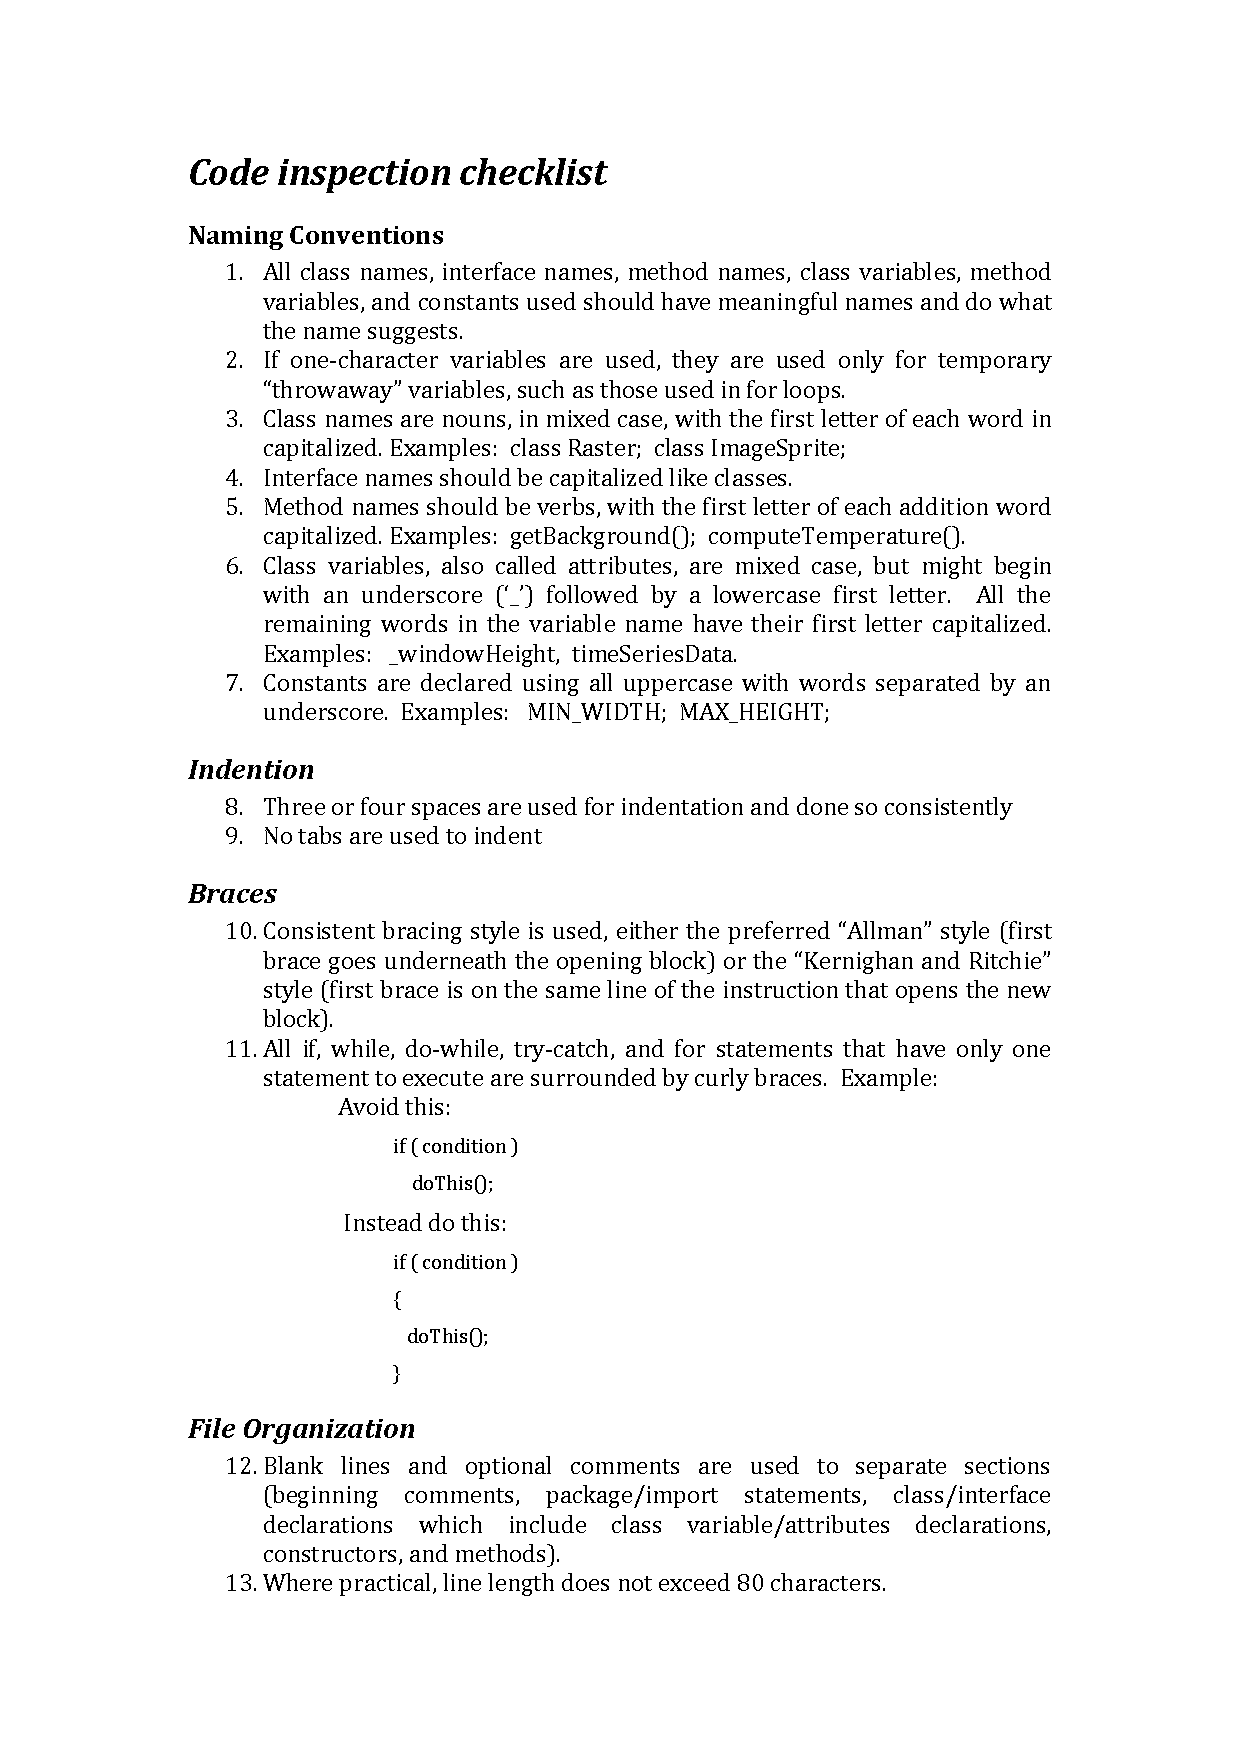
\includegraphics[page=1, width = \textwidth]{\mainpath/CodeInspectionChecklist.pdf}
\end{figure}
\begin{figure}[h!]
	\centering
	\includegraphics[page=2, width = \textwidth]{\mainpath/CodeInspectionChecklist.pdf}
\end{figure}
\begin{figure}[h!]
	\centering
	\includegraphics[page=3, width = \textwidth]{\mainpath/CodeInspectionChecklist.pdf}
\end{figure}
\begin{figure}[h!]
	\centering
	\includegraphics[page=4, width = \textwidth]{\mainpath/CodeInspectionChecklist.pdf}
\end{figure}



\end{document}